\documentclass[11pt, a4paper]{book}
% Ressources à installer : texlive-science et texlive-lang-french ou texlive-lang-european
%à compiler avec XeLaTeX à cause des image pstricks

\usepackage[utf8]{inputenc}
\usepackage[T1]{fontenc}

\usepackage[french]{babel}
\usepackage{listingsutf8}
\usepackage{pdfpages}
\usepackage{tikz,pgf}
\usepackage{amsthm,titlesec}
\usepackage{mdframed} % pour le format des définition, théorèmes...
\usepackage{xcolor,rotating,systeme}
\usepackage[Glenn]{fncychap} %pour le format des chapitres
\usepackage[top=3cm,bottom=3cm,left=3cm,right=2cm,headsep=10pt,a4paper]{geometry} % Page margins
\usepackage{multicol}
\usepackage{comment}
\usepackage{enumerate,cancel}
\usepackage{lipsum,minitoc}
%\usepackage{chngcntr}
\usepackage{amsmath,amsfonts,minitoc,amsthm,pgfplots}
\usepackage{mathrsfs}
\usetikzlibrary{arrows, intersections}
\usepackage{mathrsfs}
\usepackage{array,yhmath}
\usepackage{hyperref}
\usepackage{caption}
\usepackage{float}
\usepackage{wrapfig}
\restylefloat{figure}
%\usepackage{subfig}

\usepackage{subcaption}

\usepackage{listings}
\usepackage{color}
\lstset{ % General setup for the package
    language=Python,
    basicstyle=\footnotesize,
    basewidth=0.7em,
    numbers=left,
     numberstyle=\tiny,
    frame=lines,
    tabsize=4,
    columns=fixed,
    showstringspaces=false,
    showtabs=false,
    keepspaces,
    commentstyle=\color{gray},
    keywordstyle=\color{blue},
    stringstyle=\color{magenta},
    inputencoding=utf8/latin1,
            extendedchars=true,
            literate=%
            {é}{{\'{e}}}1
            {è}{{\`{e}}}1
            {ê}{{\^{e}}}1
            {ë}{{\¨{e}}}1
            {û}{{\^{u}}}1
            {ù}{{\`{u}}}1
            {â}{{\^{a}}}1
            {à}{{\`{a}}}1
            {î}{{\^{i}}}1
            {ô}{{\^{o}}}1
            {ç}{{\c{c}}}1
            {Ç}{{\c{C}}}1
            {É}{{\'{E}}}1
            {Ê}{{\^{E}}}1
            {À}{{\`{A}}}1
            {Â}{{\^{A}}}1
            {Î}{{\^{I}}}1
    }



\usepackage{lipsum}
\newtheorem{example}{Exemple}

\usepackage{pstricks,pst-plot,pstricks-add}
\usepackage{pst-func,tkz-tab,tkz-euclide}
\usepackage{graphicx}
%macro exo
\newcounter{mtex}[chapter]
\newcommand{\mtexlabel}{\cadrexo{\themtex}}
\newcommand{\cadrexo}[1]{%
\tikz\node[rectangle,minimum size=6mm,rounded corners=2mm,fill=ocre,inner sep=0pt,text width=0.8cm,align=center]{\large\bfseries\textcolor{white}{#1}};}
\definecolor{ocre}{RGB}{196,106,106}
\definecolor{vert}{RGB}{55,120,0}
\newcommand{\mtexlabelpos}[1]{%
\makebox[0pt][r]{\raisebox{#1\baselineskip}[0pt][0pt]{\mtexlabel\quad}}}
\newenvironment{exercice}[1][\empty]{%
\refstepcounter{mtex}%
\trivlist\item\relax%  
\ifx#1\empty\mtexlabelpos{-.7}\else\mtexlabelpos{-.5}%
\hfill\textbf{#1}\hfill\mbox{}\par\fi%
}{\endtrivlist}

\newcommand{\N}{\mathbb{N}}
\newcommand{\Z}{\mathbb Z}
\newcommand{\Q}{\mathbb Q}
\newcommand{\R}{\mathbb R}
\newcommand{\C}{\mathbb C}

\newcommand{\ssi}{\;\;\Leftrightarrow\;\;}

\newcommand{\point}[1]{-- +(#1,#1) -- +(-#1,-#1) -- +(0,0) -- +(-#1,#1) -- +(#1,-#1)} 


\newcommand{\parallele}{\mathbin{\!/\mkern-5mu/\!}} %signe parallèle

\titleformat{\chapter}[frame]
{\setlength\fboxrule{2.25pt}\color{black}}%
{\filleft\scshape\LARGE%
\enspace  Chapitre \thechapter\enspace}%
{20pt}
{\rule{0pt}{30pt}\Huge\scshape\filleft}

\newcommand\fonction[5]{
$\begin{array}{rrll}
#1: & #2 & \rightarrow & #3 \\
  & #4 & \mapsto & #5
\end{array}$
}

%\titleformat
%{\section} % command
%[hang] % shape
%{\bfseries\Large} % format
%{ \thesection\quad} % label
%{0em} % sep
%{
%} % before-code
%[
%\vspace{-1ex}%
%\textcolor{blue!60}{\rule{10cm}{3pt}}
%] % after-code


%\theoremstyle{break}
\newtheoremstyle{definition-style}  %style des theoreme
{}               
{}               
{}                   
{}                   
{\bf\sffamily} 
{~:\\[0.3cm]}                 
{.5em}               
{\thmname{#1}\thmnumber{ #2}\thmnote{ (#3)}}

\mdfdefinestyle{defi-frame}{
linewidth=10pt, %
linecolor= blue!50, % 
backgroundcolor= blue!20,
topline=false, %
bottomline=false, %
rightline=false,%
leftmargin=0pt, %
innerleftmargin=15pt, %
innerrightmargin=1em, 
rightmargin=0pt, % 
innertopmargin=-2pt,%
innerbottommargin=6pt, % 
splittopskip=\topskip, %
%splitbottomskip=\topskip, %
}% 

\mdfdefinestyle{methode-frame}{
	linewidth=10pt, %
linecolor= gray!70, % 
backgroundcolor= white,
topline=false, %
bottomline=false,%
rightline=false,%
leftmargin=0pt, %
innerleftmargin=15pt, %
innerrightmargin=1em, 
rightmargin=0pt, % 
innertopmargin=-2pt,%
innerbottommargin=6pt, % 
splittopskip=\topskip, %
%splitbottomskip=\topskip, %
}% 


\mdfdefinestyle{thm-frame}{
linewidth=10pt, %
linecolor= red!50, % 
backgroundcolor= orange!30,
topline=false, %
bottomline=false, %
rightline=false,%
leftmargin=0pt, %
innerleftmargin=15pt, %
innerrightmargin=1em, 
rightmargin=0pt, % 
innertopmargin=-2pt,%
innerbottommargin=6pt, % 
splittopskip=\topskip, %
%splitbottomskip=\topskip, %
}% 

\mdfdefinestyle{lem-frame}{
linewidth=10pt, %
linecolor= yellow!50, % 
backgroundcolor= yellow!10,
topline=false, %
bottomline=false, %
rightline=false,%
leftmargin=0pt, %
innerleftmargin=15pt, %
innerrightmargin=1em, 
rightmargin=0pt, % 
innertopmargin=-2pt,%
innerbottommargin=6pt, % 
splittopskip=\topskip, %
%splitbottomskip=\topskip, %
}% 

\mdfdefinestyle{notation-frame}{
linewidth=10pt, %
linecolor= blue!30, % 
backgroundcolor= blue!10,
topline=false, %
bottomline=false, %
rightline=false,%
leftmargin=0pt, %
innerleftmargin=15pt, %
innerrightmargin=1em, 
rightmargin=0pt, % 
innertopmargin=-2pt,%
innerbottommargin=6pt, % 
splittopskip=\topskip, %
%splitbottomskip=\topskip, %
}% 

\mdfdefinestyle{remarque-frame}{
linewidth=0pt, %
linecolor= black!0, % 
backgroundcolor= blue!0,
topline=false, %
bottomline=false, %
rightline=false,%
leftmargin=0pt, %
innerleftmargin=25pt, %
innerrightmargin=25pt, 
rightmargin=0pt, % 
innertopmargin=-2pt,%
innerbottommargin=6pt, % 
splittopskip=\topskip, %
%splitbottomskip=\topskip, %
}% 
\surroundwithmdframed[style=defi-frame]{defi}

\surroundwithmdframed[style=thm-frame]{thm}

\surroundwithmdframed[style=lem-frame]{lem}

\surroundwithmdframed[style=notation-frame]{notation}

\surroundwithmdframed[style=remarque-frame]{remarque}

\surroundwithmdframed[style=remarque-frame]{remarques}

\surroundwithmdframed[style=methode-frame]{methode}

\theoremstyle{definition-style}

%pour avoir un compteur commun a remarque et remarques
\newcounter{compteurremarque}[chapter]
\renewcommand{\thecompteurremarque}{\arabic{compteurremarque}} %définition de l'affichage du compteur

\newtheorem{defi}{Définition}[chapter]
\renewcommand{\thedefi}{\arabic{defi}} %pour ne pas avoir le numéro du chapitre dans la numération de la def
\newtheorem{thm}{Théorème}[chapter]
\renewcommand{\thethm}{\arabic{thm}}
\newtheorem{lem}{Lemme}[chapter]
\renewcommand{\thelem}{\arabic{lem}}
\newtheorem{notation}{Notation}[chapter]
\renewcommand{\thenotation}{\arabic{notation}}
%\newtheorem{remarque}{Remarque}[chapter]
%\renewcommand{\theremarque}{\arabic{remarque}}
%\newtheorem{remarques}{Remarques}[chapter]
%\renewcommand{\theremarques}{\arabic{remarques}}
\newtheorem{methode}{Méthode}[chapter]
\renewcommand{\themethode}{\arabic{methode}}


\newtheorem{remarque}[compteurremarque]{Remarque}
\newtheorem{remarques}[compteurremarque]{Remarques} %remarque et remarques prennent compteurremarque comme compteur commun

\lstMakeShortInline[columns=fixed]|

%%%%%%%% Commandes de Matthieu

%-------------------------------------------------------------------------------
%---- Eclairage : en encadré sur fond jaune avec symbôle "ampoule" à gauche ----
%-------------------------------------------------------------------------------
\definecolor{coleclairage}{RGB}{255 , 221 , 156}
\definecolor{contoureclairage}{RGB}{255 , 192 , 0}
\newenvironment{eclairage}
{
	\begin{center}%
		\begin{tikzpicture}%
			\node[rectangle, draw=contoureclairage, top color=coleclairage!50, bottom color=coleclairage!140, rounded corners=5pt, inner xsep=5pt, inner ysep=6pt, outer ysep=10pt]\bgroup                     
			\begin{minipage}{0.98\linewidth}
				\begin{minipage}{0.08\linewidth}\centerline{
\includegraphics[scale=1]{images/Symbole_eclairage.png}}\end{minipage}
				\begin{minipage}{0.89\linewidth}\itshape\footnotesize
				}
				{                		
				\end{minipage}
			\end{minipage}\egroup;%
		\end{tikzpicture}%
	\end{center}%
}



\newcommand{\putfigure}[6]{
    \begin{minipage}{#1\textwidth}
    \centering
        \includegraphics[width=#2\textwidth,height=#3\textheight]{#4}
        \captionof{figure}{#5}
        \label{#6}
    \end{minipage}
}


\newcommand{\itemb}[1]{\item \textbf{#1}}



%-------------------------------------------------------------------------------
%---- apprendre : en encadré sur fond jaune avec symbole "ampoule" à gauche ----
%-------------------------------------------------------------------------------
\definecolor{colapprendre}{RGB}{50,205,50}
\definecolor{contourapprendre}{RGB}{34,139,34}
\newenvironment{apprendre}
{
	\begin{center}%
		\begin{tikzpicture}%
			\node[rectangle, draw=contourapprendre, top color=colapprendre!10, bottom color=colapprendre!50, rounded corners=5pt, inner xsep=5pt, inner ysep=6pt, outer ysep=10pt]\bgroup                     
			\begin{minipage}{0.98\linewidth}
				\begin{minipage}{0.08\linewidth}\centerline{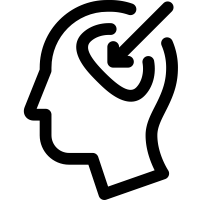
\includegraphics[width=30px]{images/Symbole_learn.png}}\end{minipage}
				\begin{minipage}{0.89\linewidth}\itshape\footnotesize
				}
				{                		
				\end{minipage}
			\end{minipage}\egroup;%
		\end{tikzpicture}%
	\end{center}%
}

\definecolor{colimportant}{RGB}{247 , 189 , 164}
\definecolor{contourimportant}{RGB}{237 , 125 , 49}
\newenvironment{important}
{
	\begin{center}%
		\begin{tikzpicture}%
			\node[rectangle, draw=contourimportant, top color=colimportant!50, bottom color=colimportant!140, rounded corners=5pt, inner xsep=5pt, inner ysep=6pt, outer ysep=10pt]\bgroup                     
			\begin{minipage}{0.08\linewidth}\centerline{
\includegraphics[scale=0.8]{images/Symbole_attention.png}}\end{minipage}
			\begin{minipage}{0.89\linewidth}
			}
			{                		
			\end{minipage}\egroup;
		\end{tikzpicture}%
	\end{center}%
}

%----------------------------------------------
\newcounter{compteurmonprogramme}
\setcounter{compteurmonprogramme}{1}
\newenvironment{monprogramme}
{
	\begin{center}%
		\begin{tikzpicture}%
			\node[rectangle, draw=black, rounded corners=5pt, inner xsep=5pt, inner ysep=6pt, outer ysep=10pt]\bgroup                     
			\begin{minipage}{0.98\linewidth}
				{\bf Programme \thechapter.\thecompteurmonprogramme\;:}
				
				\vspace{2mm}\hspace{7.5mm}
				\begin{minipage}{0.93\linewidth}
				}
				{                		
				\end{minipage}
				\stepcounter{compteurmonprogramme}
			\end{minipage}\egroup;%
		\end{tikzpicture}%
	\end{center}%
}



%------------------------------------------------
%---- Définition : en encadré sur fond blanc ----
%------------------------------------------------
\newcounter{compteurdef}
\setcounter{compteurdef}{1}
\newenvironment{mydefinition}
{
	\begin{center}%
	\begin{tikzpicture}%
		\node[rectangle, draw=black, rounded corners=5pt, inner xsep=5pt, inner ysep=6pt, outer ysep=10pt]\bgroup                    
		\begin{minipage}{0.98\linewidth}
			{\bf {\underline {Définition \thechapter.\thecompteurdef}}}
			
			\vspace{2mm}\hspace{4.5mm}
			\begin{minipage}{0.93\linewidth}
			}
			{                		
			\end{minipage}
			\stepcounter{compteurdef}
		\end{minipage}\egroup;%
	\end{tikzpicture}%
\end{center}%
}

\newenvironment{mydefinitions}
{
	\begin{center}%
		\begin{tikzpicture}%
			\node[rectangle, draw=black, rounded corners=5pt, inner xsep=5pt, inner ysep=6pt, outer ysep=10pt]\bgroup                    
			\begin{minipage}{0.98\linewidth}
				{\bf {\underline {Définitions \thechapter.\thecompteurdef}}}
				
				\vspace{3mm}\hspace{4.5mm}
				\begin{minipage}{0.93\linewidth}\slshape
					\begin{itemize}\setlength{\itemsep}{1mm}
					}
					{                		
				\end{itemize}\end{minipage}
				\stepcounter{compteurdef}
			\end{minipage}\egroup;%
		\end{tikzpicture}%
	\end{center}%
}



%------------------------------------------------
%---- Exemple : en encadré sur fond blanc ----
%------------------------------------------------
\newcounter{compteurex}
\setcounter{compteurex}{1}
\newenvironment{myexample}{
	\begin{center}
	\vspace{-3mm}
	\begin{minipage}{1\linewidth}
		\vspace{2mm}
		{\textsl {\underline {Exemple \thechapter.\thecompteurex}}}
		
		\vspace{2mm}\hspace{2.5mm}
		\begin{minipage}{1\linewidth}
			\begin{mdframed}[topline=false,rightline=false,bottomline=false]
}
{
			\end{mdframed}
		\end{minipage}
		\stepcounter{compteurex}
	\end{minipage}
	\end{center}
}
\newenvironment{myexamples}{
	\begin{center}
		\vspace{-3mm}
		\begin{minipage}{1\linewidth}
			\vspace{2mm}
			{\textsl {\underline {Exemples \thechapter.\thecompteurex}}}
			
			\vspace{2mm}\hspace{2.5mm}
			\begin{minipage}{1\linewidth}%\slshape
				\begin{mdframed}[topline=false,rightline=false,bottomline=false]
					\begin{enumerate}\setlength{\itemsep}{1mm}
				}
				{
					\end{enumerate}
				\end{mdframed}
			\end{minipage}
			\stepcounter{compteurex}
		\end{minipage}
	\end{center}
}



\newtheorem*{question}{Question}



%%%%%%%%%%%%%%%%%%%%%%%%%%%%%%%%%%%%%%%%%%%%%%%%%%%%%%%%%%%%%%%%%%%%%%%%%%%%
%%%%%%%%%%%%%%%%%%%%%%%%%%%   LABELS activite   %%%%%%%%%%%%%%%%%%%%%%%%%%%
%%%%%%%%%%%%%%%%%%%%%%%%%%%%%%%%%%%%%%%%%%%%%%%%%%%%%%%%%%%%%%%%%%%%%%%%%%%%
\newcommand{\act}{\textbf{\textsl{Activité \arabic{compteuract}}} \vspace*{1mm}\\ \addtocounter{compteuract}{1}}
\newcommand{\actnomme}[1]{{\bf Activité \arabic{compteuract} {\textsl{\small (#1)}}}\vspace*{1mm}\\  \addtocounter{compteuract}{1}}
\newcounter{compteuract}
\setcounter{compteuract}{1}
\newcommand{\getactcompteur}{{\the\numexpr \arabic{compteuract} - 1 \relax}}



%%%%%%%%%%%%%%%%%%%%%%%%%%%%%%%%%%%%%%%%%%%%%%%%%%%%%%%%%%%%%%%%%%%%%%%%%%%%
%%%%%%%%%%%%%%%%%%%%%%%%%%%   LABELS EXERCICES   %%%%%%%%%%%%%%%%%%%%%%%%%%%
%%%%%%%%%%%%%%%%%%%%%%%%%%%%%%%%%%%%%%%%%%%%%%%%%%%%%%%%%%%%%%%%%%%%%%%%%%%%
\newcommand{\exo}{\textbf{\textsl{Exercice \arabic{compteurexo}}} \vspace*{1mm}\\ \addtocounter{compteurexo}{1}}
\newcommand{\exonomme}[1]{{\bf Exercice \arabic{compteurexo} {\textsl{\small (#1)}}}\vspace*{1mm}\\  \addtocounter{compteurexo}{1}}
\newcommand{\eexo}{\vspace{5mm}} % espace pour séparer les exercices
\newcounter{compteurexo}
\setcounter{compteurexo}{1}
\newcommand{\getexocompteur}{{\the\numexpr \arabic{compteurexo} - 1 \relax}}
\usepackage{minted}
\pgfplotsset{compat=1.17}
\begin{document}

\setcounter{chapter}{2}

\chapter{Notion de fichiers}

\section{Fichiers}
\subsection{Introduction}

Un fichier informatique est un ensemble de données numériques que l'on souhaite faire persister en le stockant sur un support permanent. Un fichier peut être :une image, un film, du texte, un programme source, un programme exécutable, un fichier compressé, etc. Quant au support permanent (cf. chapitre Ordinateur) il s'agit d'un disque dur, un DVD, une clé USB, etc.

Un disque stocke simplement une suite de bits, une suite de 0 et de 1. Le nombre de bits qu’un disque peut stocker est appelé sa capacité : par exemple un disque d’un téraoctet (binaire) peut stocker 240 mots de 8 bits, soit un peu plus de huit mille milliards de bits. On peut donc facilement stocker un texte, une image, un son ou un programme sur un tel disque. Cependant, comme on souhaite souvent stocker sur un disque plusieurs images, textes, etc., il faut diviser les huit mille milliards de bits dont le disque est constitué en plusieurs espaces plus petits, que l’on appelle des fichiers. Un fichier est simplement une suite de 0 et de 1, à laquelle on associe un nom. Par exemple, le texte "\textit{Je pense, donc je suis.}" se représente en ASCII étendu comme la suite de 184 bits suivante :

\begin{minted}{latex}
0100101001100101001000000111000001100101011011
1001110011011001010010110000100000011001000110
1111011011100110001100100000011010100110010100
1000000111001101110101011010010111001100101110
\end{minted}

Il est possible de stocker cette suite de bits sur un disque en lui donnant le nom \texttt{cogito.txt}, l’extension txt indiquant que cette suite de bits exprime un texte en ASCII. L’extension détermine le type d’information exprimé (texte, image, son, etc.) et le format utilisé pour l’exprimer.

\subsection{Nom de fichier}
Un fichier comporte donc un {\it nom\_de\_fichier}  qui permet de l’identifier et d’y accéder. Ce nom est généralement constitué de deux parties séparées par un point. Par exemple, le fichier nommé {\it Recette\_tarte\_aux\_pommes.odt} se décompose :

\begin{center}
\begin{tikzpicture}
	\filldraw[fill=lightgray] (0,0.8) rectangle (10,1.6);
	\draw (0,0) rectangle (10,0.8)
			(0,0) rectangle (10,1.6)
			(0,0) rectangle (5,1.6)
			(0,0) rectangle (7.5,1.6);
	\draw (2.5,1.2) node {\bf Nom du fichier};
	\draw (6.25, 1.2) node {\bf .};
	\draw (8.75,1.2) node {\bf Extension};
	
	\draw (2.5,0.4) node {\it Recette\_tarte\_aux\_pommes};
	\draw (6.25, 0.4) node {\bf .};
	\draw (8.75,0.4) node {\it odt};
			
\end{tikzpicture}
\end{center}

Comme le nom du fichier identifie son contenu, il est important de choisir un nom explicite. En effet, si vous nommez votre rédaction de français avec le nom suivant :

$\rightarrow$ {\it Rédaction\_le\_petit\_prince.odt} : Ce fichier désignera probablement une rédaction avec comme sujet le petit prince.

Par contre, si vous choisissez le nom :

$\rightarrow$ {\it mon\_fichier.odt} : Ce nom ne donne aucune information sur son contenu. On n’aura strictement aucune idée de quoi il s’agit sauf qu’il s’agit d’un fichier !
\begin{remarques}
\begin{enumerate}
\item[]
\item Pour l’utilisateur·trice, il est donc utile et important de bien choisir un nom qui identifie le contenu de son fichier.
\item Vous remarquez également que des caractères soulignés ( \_ ) ont été utilisés dans la nomenclature. En effet, pendant longtemps, les espaces n’étaient pas autorisés pour nommer des fichiers, car les espaces étaient utilisés comme séparateurs de nom de fichier ! Actuellement, l’espace est accepté sur la plupart des systèmes, mais il existe toujours de vieux programmes qui refusent un espace dans le nom du fichier ou génère une erreur.
\item Les caractères accentués (é ê è ü à ä î ô û) étaient également interdits. C’est pour cette raison que l’on trouve souvent des fichiers qui n’ont pas d’accent (merci l’orthographe me direz-vous). À noter qu’il subsiste également d’autres caractères qui sont interdits ou déconseillés:
\begin{itemize}
\item Microsoft Windows (interdits) $< \; >  \,  :  \;   " \;   \backslash \;  / \; \vert \; . \; ? \; *$ 
\item Gnu/Linux et Mac OS (déconseillés): $/$ * 
\end{itemize}
\item Les noms ont aussi une limite en longueur, jusqu’à 256 caractères (voir plus pour les tout nouveaux systèmes), mais dans les années 80, le système d’exploitation MS-Dos n’autorisait que 8 caractères plus le point et l’extension de 3 caractères !
\item Certains systèmes de fichier sont sensibles à la casse, mais pas Microsoft Windows. Exemple avec ces trois noms :
\begin{enumerate}[a)]
\item {\it recette\_tarte\_aux\_pommes.odt}
\item {\it Recette\_tarte\_aux\_pommes.odt}
\item {\it RECETTE\_TARTE\_AUX\_POMMES.odt}
\end{enumerate}
Ces trois fichiers indiqueront le même document pour Microsoft Windows, mais bien trois fichiers distincts pour GNU/Linux ou macOS.
\end{enumerate}
\end{remarques}

\section{Extension}
\subsection{Type d'extension}
Comme cité précédemment, l’extension est formée en général de 3 lettres, mais elle peut en contenir plus (ex. : .html), voir moins ou carrément aucune. L’extension, par convention, indique la nature du fichier. Voici quelques exemples :

\begin{center}
\begin{tikzpicture}
	\filldraw[fill=lightgray] (0,8.8) rectangle (12,8);
	\draw (12,-.8) rectangle
	(0,0) rectangle (12,0.8) rectangle (0,1.6) 
		rectangle (12,2.4) rectangle (0,3.2) 
		rectangle (12,4) rectangle (0,4.8)
		rectangle (12,5.6) rectangle (0,6.4)
		rectangle (12,7.2) rectangle (0,8);
	\draw (8,-0.8) -- (8,8.8);
	
	\draw (4,8.4) node {\bf Nature du contenu};
	\draw (10,8.4) node {\bf Extensions};
	
	\draw (4,7.6) node {Document texte libre office writer};
	\draw (10,7.6) node { odt};
	
	\draw (4,6.8) node {Document tableur libre office calc};
	\draw (10,6.8) node {ods};
	
	\draw (4,6) node {Document texte Microsoft Word};
	\draw (10,6) node {docx};
	
	\draw (4,5.2) node {Document tableur Microsoft Excel};
	\draw (10,5.2) node {xlsx};
	
	\draw (4,4.4) node {Document texte};
	\draw (10,4.4) node {txt};
	
	\draw (4,3.6) node {Exemples de formats de fichiers compressés};
	\draw (10,3.6) node {zip, 7z, rar, lzw};
	
	\draw (4,2.8) node {Exemples de formats de fichiers audio};
	\draw (10,2.8) node {mp3, wav, ogg, flac};
	
	\draw (4,2) node {Images, photos};
	\draw (10,2) node {png, jpeg, gif};
	
	\draw (4,1.2) node {Video, film};
	\draw (10,1.2) node {avi, mpg, mov, flv};
	
	\draw (4,0.4) node {Page web};
	\draw (10,0.4) node {htm, html};
	
	\draw (4,-0.4) node {Exemples de formats de fichiers de code source};
	\draw (10,-0.4) node {java, c, py};

\end{tikzpicture}
\end{center}
\begin{comment} % ce chapitre ne me semble pas très pertinent 
\subsection{Type MIME}
Les systèmes d'exploitation gnu/Linux et MacOS ne demandent pas d'extension aux différents type de fichiers. En effet, ces deux systèmes se basent sur des informations rattachées aux fichiers, les types MIME. Les types MIME sont désormais appelés "types de média Internet". Les types MIME ont été créés à l’origine pour le courrier électronique. "MIME" (Multipurpose Internet Mail Extensions) est un standard qui a été proposé par les laboratoires Bell Communications en 1991 afin d'étendre les possibilités du courrier électronique (courriel), c'est-à-dire de permettre d'insérer des documents (images, sons, texte, ...) lors d'un envoi de message électronique, mais ils se sont étendus à d’autres utilisations.

MS Windows ignore les types MIME et se base uniquement sur les extensions de fichier. Par exemple, vous pouvez avoir un fichier texte nommé "Exemple.txt". MS Windows comprend qu’il s’agit d’un fichier texte en raison de l’extension de fichier .txt. Supprimez le .txt. extension de fichier et renommer le fichier en "Exemple" sans extension de fichier. MS Windows ne saura pas quoi faire avec le fichier résultant. C’est pourquoi MS Windows vous avertit lors de la suppression de l’extension de fichier, en disant "Si vous modifiez une extension de nom de fichier, le fichier peut devenir inutilisable. Êtes-vous sûr de vouloir le changer ?". 
\begin{figure}[h!]
\centering
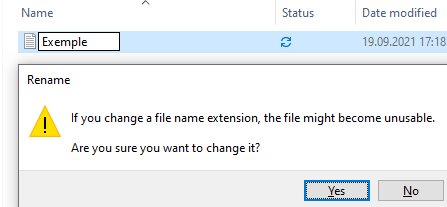
\includegraphics[width=10cm]{images/change_extension.png}
\end{figure}

Ce fichier ne deviendra pas inutilisable (pour toujours). Vous pouvez le rendre à nouveau "utilisable" en ajoutant l’extension du fichier d’origine.
C’est une des raisons principales de MS Windows de masquer les extensions de fichiers par défaut dans son explorateur de fichier. Cette option évite que les utilisateurs suppriment accidentellement l'extension d'un fichier. Des attaquants (pirates) peuvent abuser de ce comportement pour cacher du code malveillant et des virus dans des fichiers en choisissant de fausses extensions de fichiers.

Les informations sur la nature du fichier, le type MIME, sont intégrées au début du fichier lui-même. Ainsi, lorsque vous ouvrez un fichier sans extension de fichier, gnu/Linux et MacOS examineront le type MIME du fichier pour déterminer de quel type de fichier il s’agit.
\end{comment}


\section{Organisation des fichiers}

Lorsque vous prenez une photo avec votre smartphone où se trouve-t-elle ? Quel nom de fichier identifie la photo ? Comment vous y prenez-vous pour classer vos photos ? Ne vous est-il pas arrivé de défiler les photos sur votre écran à la recherche d’une en particulier ? Comment faudrait-il procéder pour retrouver plus rapidement une photo ? Si vos photos sont classées par date et par album n’est-il pas plus simple de retrouver une photo ? Le problème dans notre cas de figure c'est que toutes les photographies se retrouvent au même endroit, sans classement, dans la mémoire permanente du téléphone mobile.

En informatique, pour organiser des fichiers, il est nécessaire de créer des dossiers (ou des répertoires). Dans un dossier, nous pouvons trouver d’autres dossiers et fichiers. Cette structure forme une hiérarchie cohérente. Organiser ses fichiers c’est comme ranger ses feuilles de cours dans plusieurs classeurs avec des pochettes et des séparateurs. Prenons l’exemple suivant pour illustrer le classement de ses feuilles de cours papier. Il s’agit donc de classer différents documents de cours dans leur classeur respectif. Dans notre illustration, nous avons choisi de créer un classeur par discipline ce qui permet, par exemple, de ranger la feuille de géographie Suisse dans la pochette Europe qui se trouve dans le classeur Géographie. Ce classeur sera rangé dans l’armoire des classeurs.

\begin{figure}[h!]
\centering
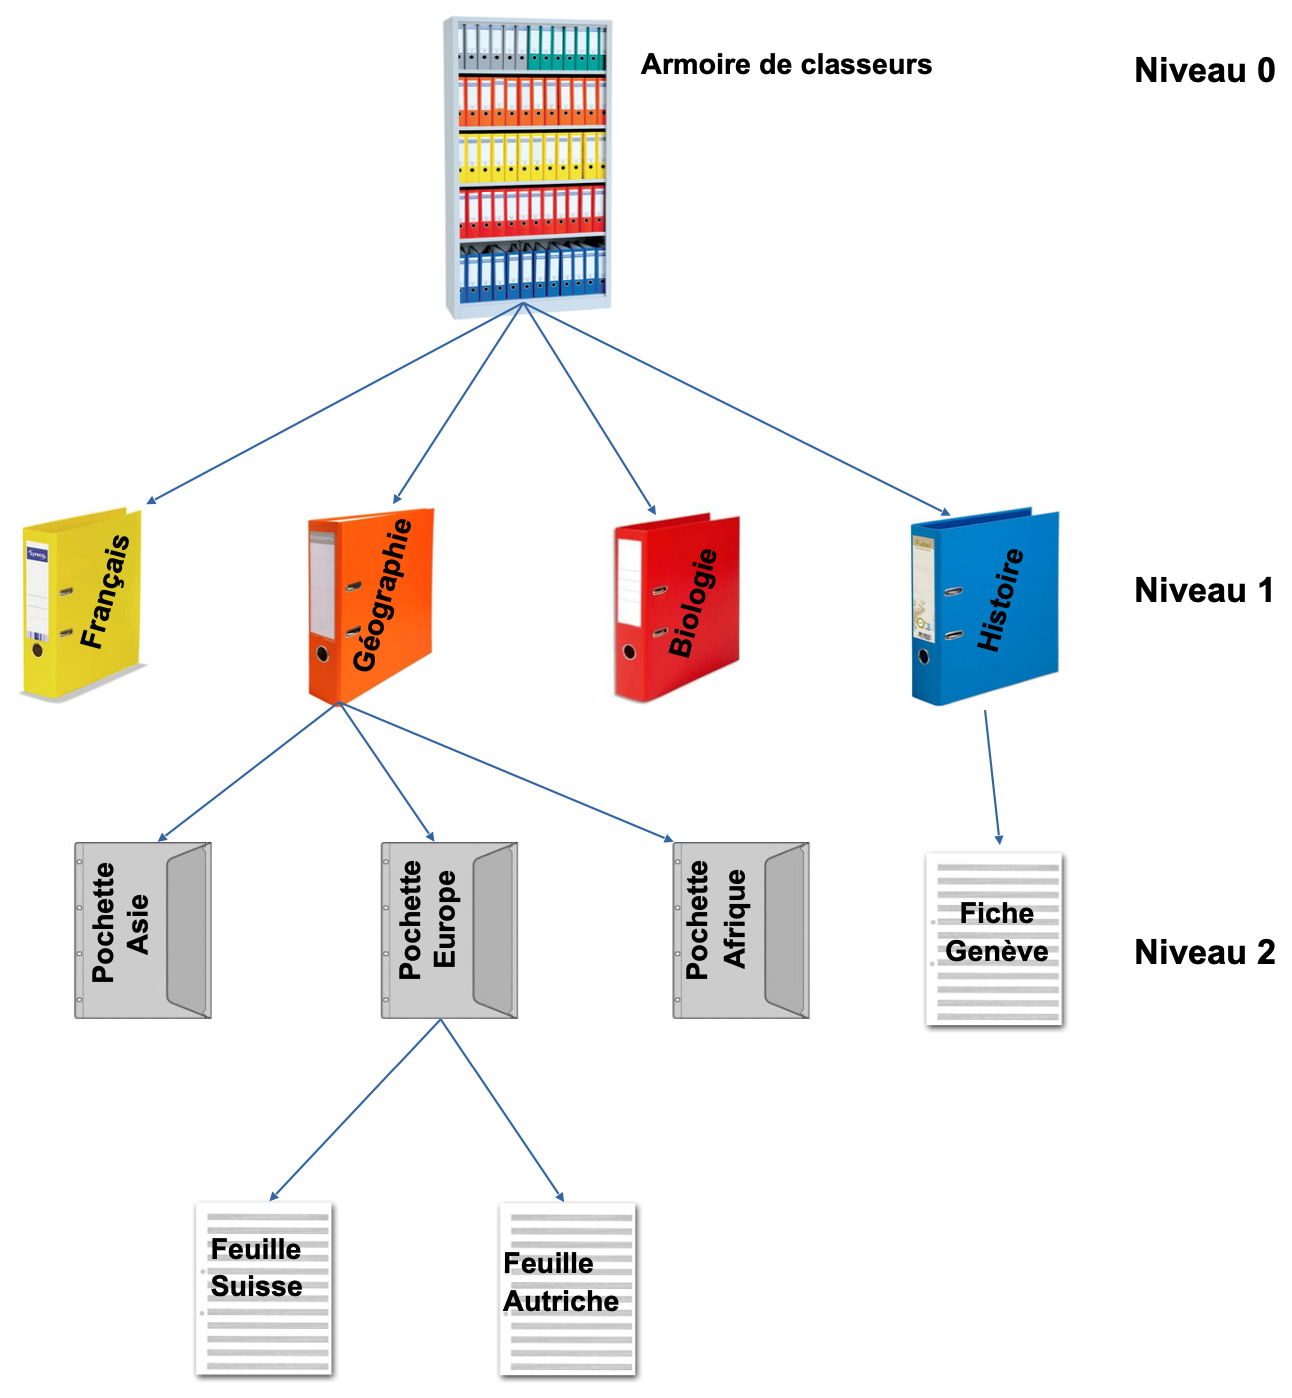
\includegraphics[width=12cm]{images/organisationfichiers}
\end{figure}

Cette structure se retrouve dans les systèmes de fichiers de manière analogue. Sous GNU/Linux ou macOS le niveau 0 se nomme la racine et le dernier niveau les feuilles (par analogie avec un arbre inversé). Le passage d’un niveau à l’autre, les branches, est décrit par un / (slash). Le chemin pour parvenir au fichier depuis la racine (niveau 0) se nomme le chemin d’accès. Il décrit précisément l’emplacement du fichier (l’itinéraire complet). On appelle une telle organisation des fichiers une organisation arborescente, car on peut la visualiser sous la forme d’un arbre.

Pour résumer: 
\begin{enumerate}[a)]
\item Un {\bf dossier} peut comporter d’autres dossiers et des fichiers.
\item Un {\bf fichier} est un ensemble organisé d'informations, désigné par un nom précis, que le système d'exploitation d'un ordinateur manipule comme une simple entité, dans sa mémoire ou sur un support de stockage.
\end{enumerate}

\begin{figure}[h!]
\centering
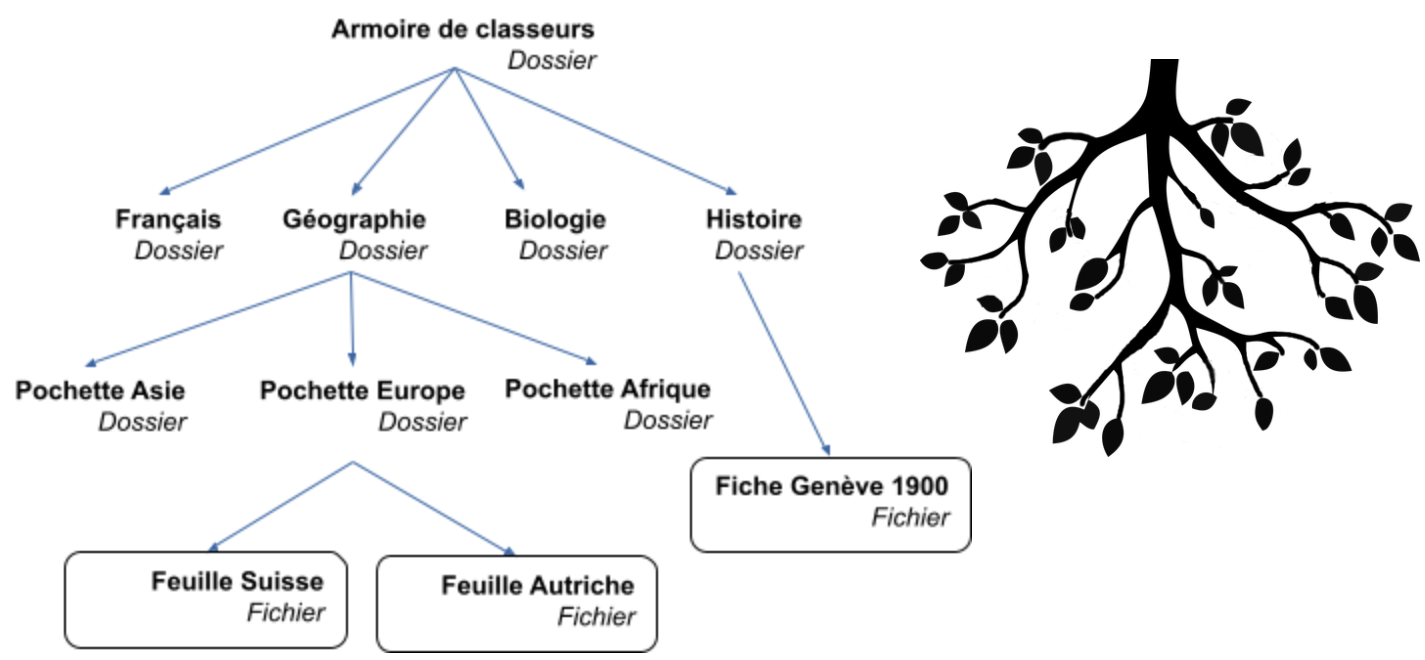
\includegraphics[width=15cm]{images/arborescence2}
\end{figure}
L’organisation arborescente des fichiers n’est pas le seul moyen de structurer l’information : elle est en concurrence avec d’autres méthodes, parmi lesquelles l’utilisation de liens hypertextes, notion qui n’a pas été inventée pour structurer l’information, mais pour simplifier le mécanisme de référence dans une page web.

% SECTION
\section{Explorateur de fichiers sous différents système d'exploitation}
Pour nous aider à parcourir l’arborescence des fichiers et des dossiers, chaque système d’exploitation offre un navigateur graphique dans son environnement graphique ou la possibilité de parcourir l'arborescence textuellement dans une console à l'aide de commande.

\subsection{MacOS et GNU/Linux}
Sous GNU/Linux et macOS, pour chercher la « Feuille Suisse.txt », on écrirait le parcours depuis la racine de manière suivante :

\begin{center}
{ \bf /Armoire de classeurs/Géographie/Pochette Europe/
}
\end{center}
\begin{figure}[h!]
         \centering
         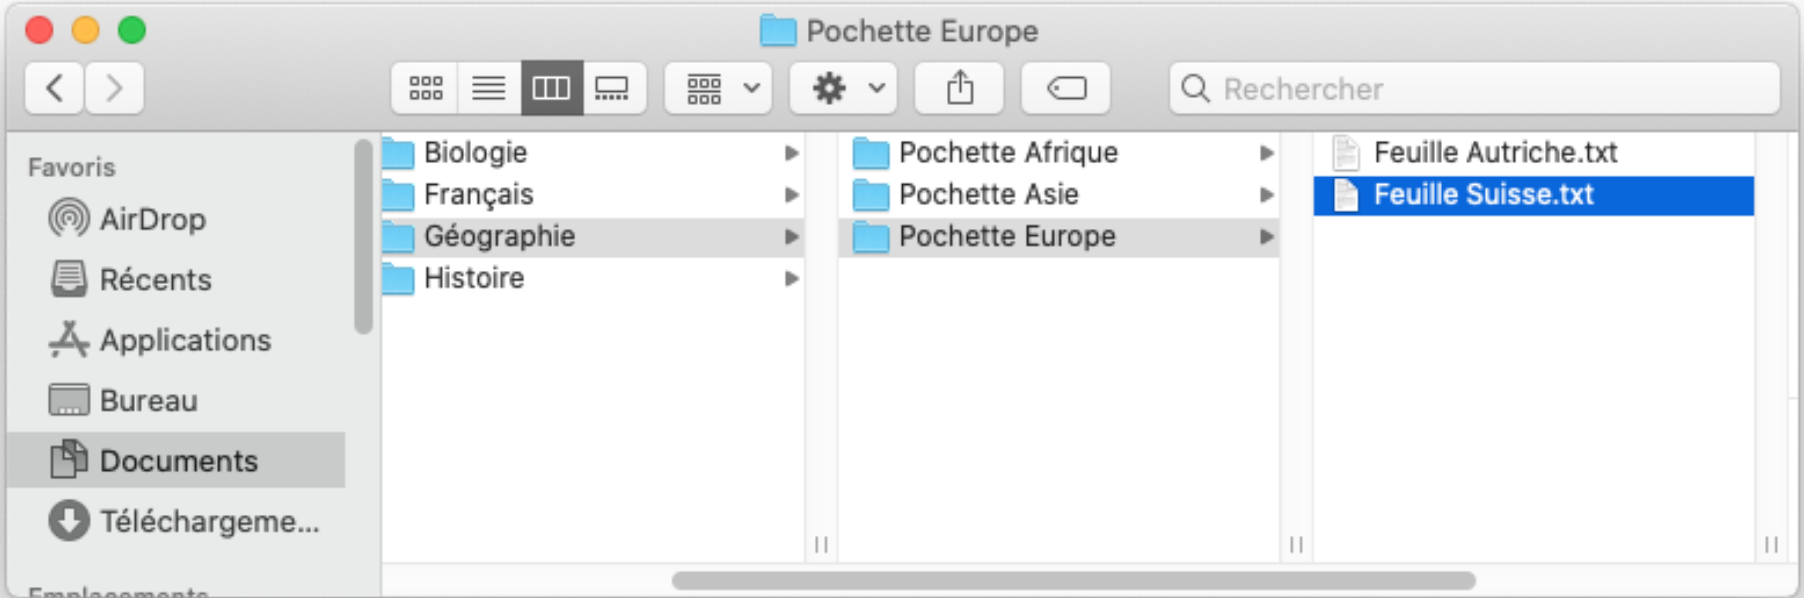
\includegraphics[width=\linewidth]{images/fichierMac}
        \caption{Système de fichiers Mac}
\end{figure}

\begin{figure}[h!]
         \centering
    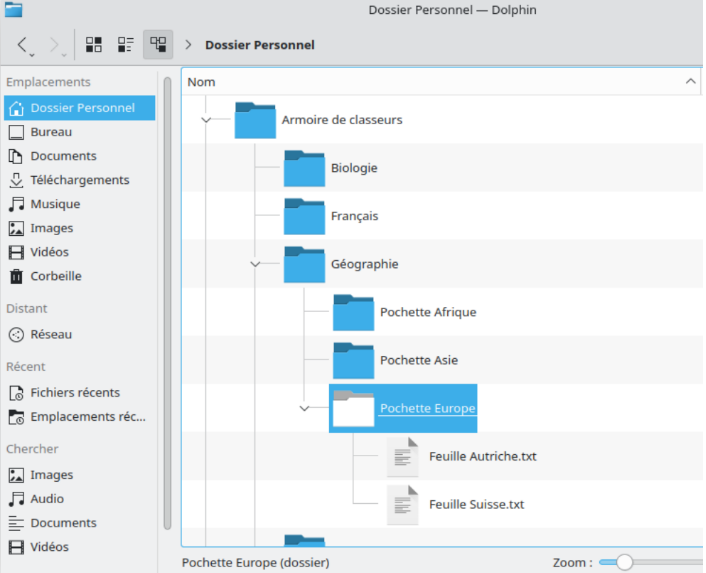
\includegraphics[width=0.7\linewidth]{images/fichiersLinux.png}
    \caption{Système de fichiers Linux}
\end{figure}

En mode console (textuel), la commande $ls$ permet de visualiser le contenu d'un répertoire et la commande $cd\ nom\_du\_dossier$ permet de se déplacer dans le dossier nommé nom\_du\_dossier.

\subsection{Microsoft Windows}

Sous Microsoft Windows, le chemin serait :

\begin{center}
{\bf C:$\backslash$Armoire de classeurs$\backslash$Géographie$\backslash$Pochette Europe
}
\end{center}

\begin{figure}[ht!]
\centering
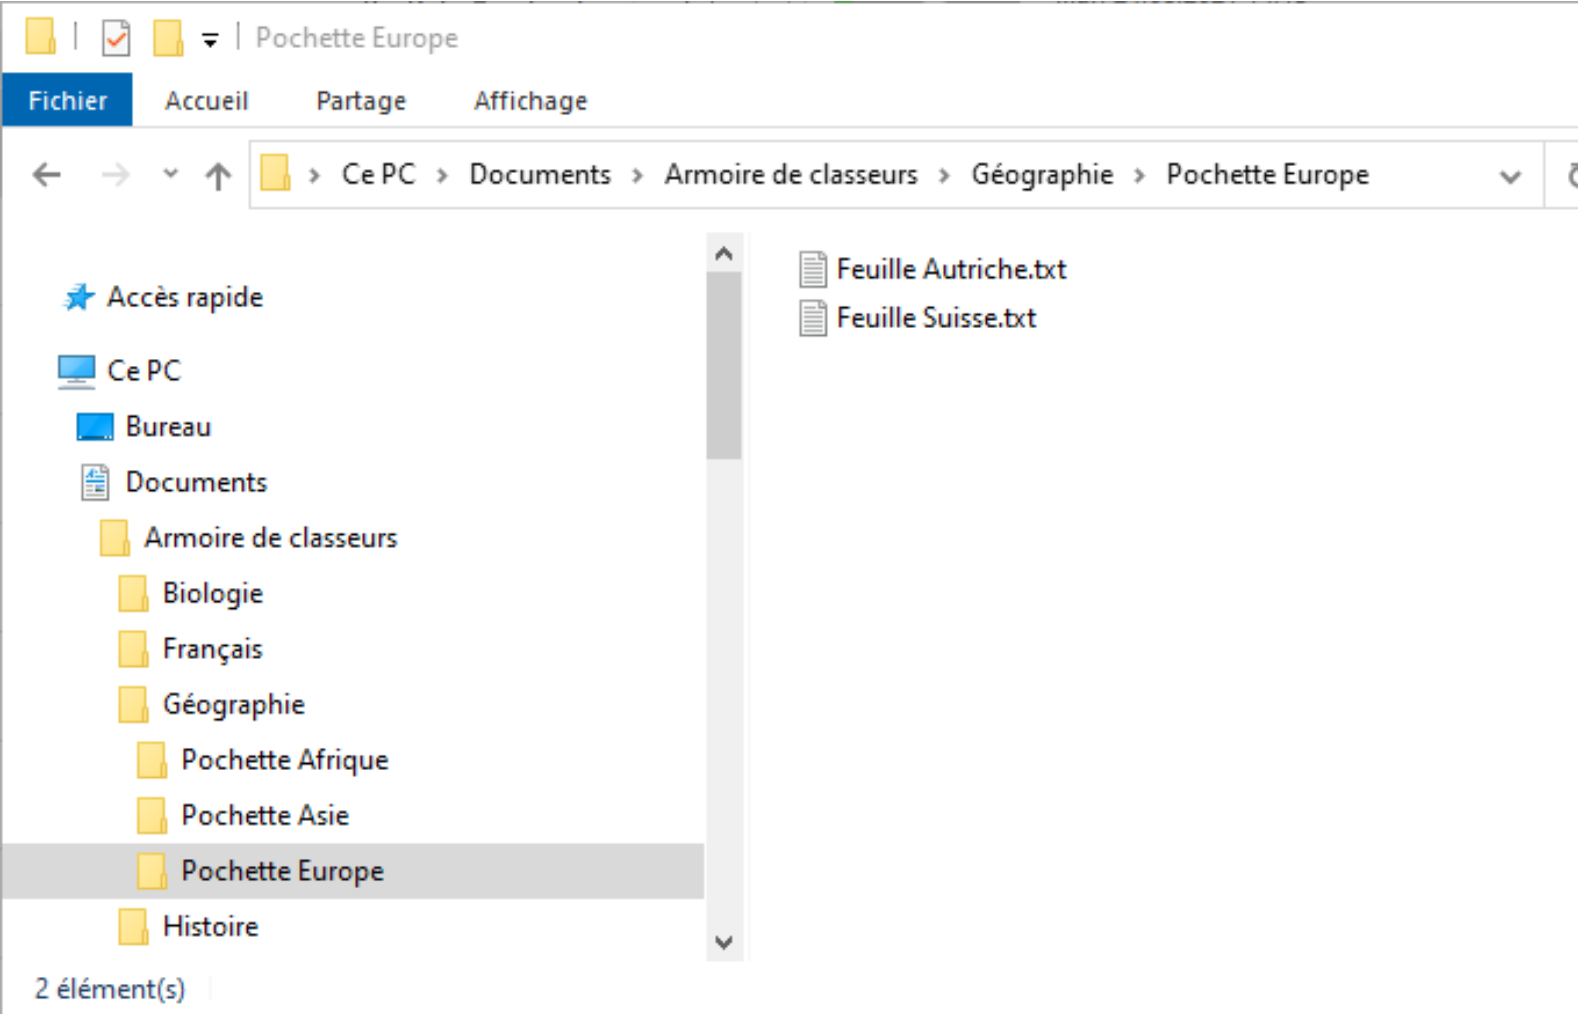
\includegraphics[width=0.7\linewidth]{images/fichierWindows}
    \caption{Système de fichiers Windows}
\end{figure}

Noter la différence entre les deux systèmes. Le caractère / qui délimite les niveaux pour GNU/Linux et macOS et le caractère $\backslash$ pour Microsoft Windows. Il y a aussi la lettre qui détermine la partition ou un périphérique (clé USB, lecteur DVD, etc.) alors que sous GNU/Linux et macOS, une partition est invisible à l’utilisateur·trice en étant considéré comme une branche de l’arbre. L'utilisation de lettre est une spécificité unique du système d'exploitation Microsoft Windows.

\section{Métadonnées}

Les \textbf{métadonnées} sont des informations décrivant: le contenu, le contexte, et les caractéristiques d'un fichier ou d'une donnée, sans être la donnée elle-même.
$\Rightarrow$ Elles permettent de mieux comprendre, organiser et rechercher des fichiers.

Exemples:
\begin{itemize}
    \item Photo numérique : Une image contient des métadonnées comme la date et l'heure de la prise de vue, les paramètres de l'appareil photo (ISO, ouverture), et la géolocalisation (où la photo a été prise).
    \item Musique : Un fichier MP3 stocke des métadonnées sur l'artiste, l'album, l'année de sortie, et la pochette d'album.
    \item Vidéo : Une vidéo peut inclure des métadonnées sur la résolution, la durée, le format de compression, et parfois le lieu de tournage.
\end{itemize}

\begin{figure}[h!]
    \centering
    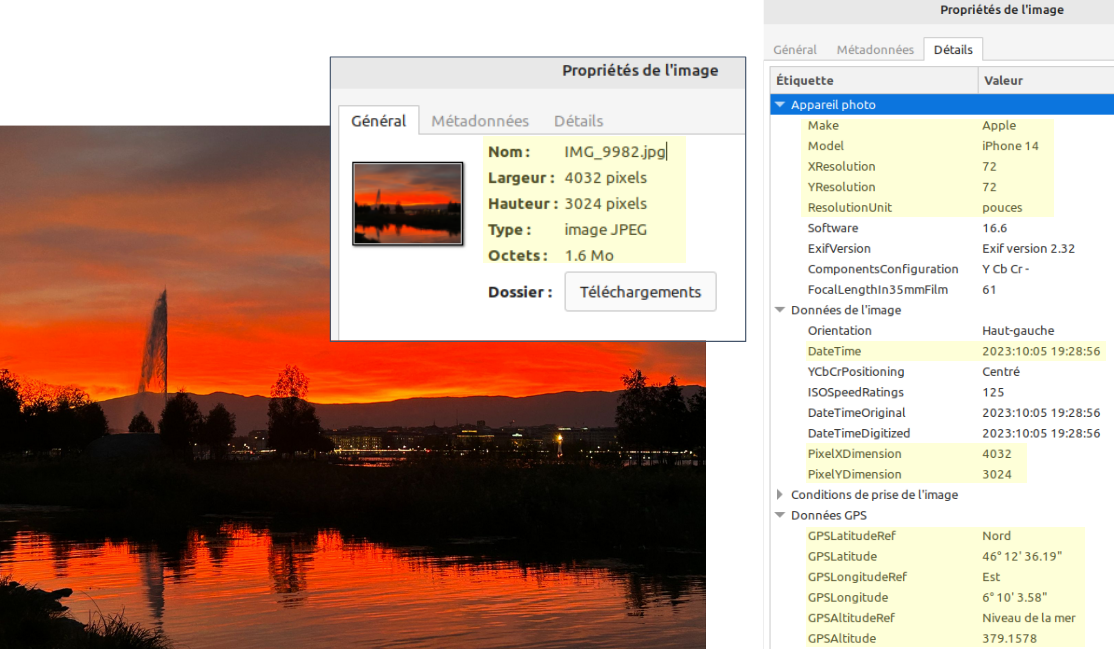
\includegraphics[width=0.75\linewidth]{images/metadata.png}
    \caption{Métadonnées d'une image}
\end{figure}


\section{Exercices}

\begin{exercice}
Se connecter sur www.eduge.ch puis aller sur le drive.
 Organiser le drive en sous fichier: Il devra y avoir un dossier principal nommé: Informatique et au moins 3 sous-dossiers appelés: Microbit, Python et Projet. 
 
 Le prochain petit programme fait en Microbit devra être sauvegardé sur le drive dans le dossier Microbit. 
\end{exercice}


\begin{exercice}
Dans moodle ou classroom, récupérez le fichier Exercice\_1\_fichier.zip et décompressez-le sur votre ordinateur.
Ouvrez le dossier "A\_Trier\_A\_Renommer", observez chaque fichier qu'il contient, renommez-les et déplacez-les dans le bon dossier. Renommez également les dossiers avec des noms corrects.
\begin{enumerate}
    \item Combien y a-t'il de dossiers dans le dossier Nourriture ?
    \item Combien y a-t'il de fichiers dans le dossier Legumes ?
    \item Quelle est la taille de l'image avec des carottes ?
    \item Quelle est l'extension de l'image avec des carottes ?
    \item Quelle est la taille du dossier Fruits ?
\end{enumerate}
\end{exercice}

\begin{exercice} *
Choisissez une photo prise avec votre smartphone. Donner quelques informations à son sujet en exploitant les métadonnées qui lui sont associées. Quand et où cette photo a-t-elle été prise? Sous quel nom et quel format est-elle stockée dans le smartphone? Quel est son poids? À quelles informations supplémentaires avons-nous accès?
\textit{Site pour lire les métadonnées : \url{https://www.verexif.com/fr/}}
\end{exercice}


\section{Stockage des données}

Les besoins en stockage de données numériques, à l’échelle mondiale, ont été multipliés par plus de vingt au cours de la dernière décennie et devraient dépasser les 50 zettaoctets ($10^{21}$) d’ici fin 2021. Comme le montre l’infographie ci-dessous, cette quantité de données apparaît finalement dérisoire en comparaison avec ce qui est attendu pour les quinze prochaines années. Les prévisions tablent en effet sur une multiplication par trois ou quatre du volume annuel de données créées tous les cinq ans. Avec ce rythme exponentiel de croissance, le seuil astronomique des 2’000 zettaoctets devrait être franchi à l’horizon 2035.

\begin{figure}[ht!]
\centering
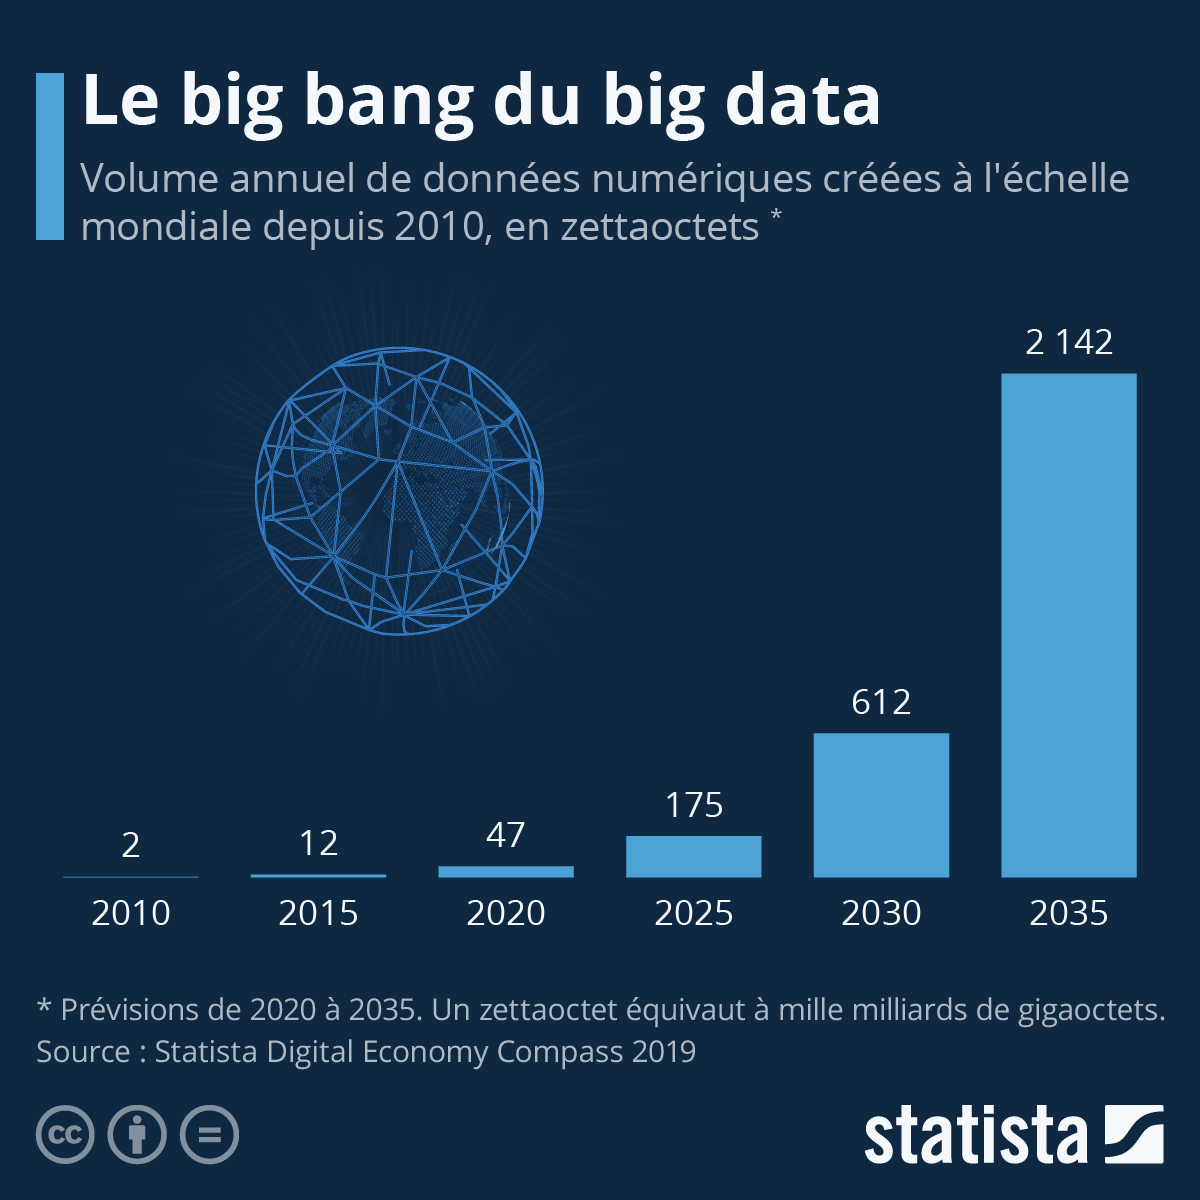
\includegraphics[width=8cm]{images/statista.jpeg}
\end{figure}

Il faudrait se procurer 500 millions de disques durs actuels (100 To) pour être capable de sauvegarder 50 [Zo] ! Cette quantité de données pose autant de problèmes de préservation et d’intégrité des données que de sauvegarde. Sans annoncer les problèmes de places, de consommation électrique, de pollutions dues à la fabrication et au recyclage du matériel vieillissant, de coût et de sauvegarde.

\section{Octet : unités de mesure en informatique}
Rappel : un octet permet de représenter $2^8$ nombres, soit 256 valeurs différentes.
\begin{center}
   \begin{tabular}{| r || c |  c | c | c | c | c | c |  c |}
     \hline
     Symbole & ko & Mo & Go & To & Po & Eo & Zo & Yo \\ \hline
     Nom & kilooctet & mégaoctet & gigaoctet & téraoctet & pétaoctet & exaoctet & zettaoctet & yottaoctet   \\ \hline
     Valeur & $10^{3}$ & $10^{6}$ & $10^{9}$ & $10^{12}$ & $10^{15}$ & $10^{18}$ & $10^{21}$ & $10^{24}$  \\ \hline
   \end{tabular}
\end{center}

Exemples de tailles de fichier (ordre de grandeur):
\begin{enumerate}
    \item[-] 2 Ko :        fichier texte (2’000 lignes de texte)
    \item[-] 1 à 20 Mo :    photo compressée (jpeg) d’un appareil photo numérique.
    \item[-] 10 Mo :     fichier MP3 d’une durée ~5 min (débit 320 kbit/s)
    \item[-] 700 Mo :     film ~1h30 (compression – qualité DVD)
    \item[-] 3 Go :         film ~1h30 (compression – qualité Blu-ray)
    \item[-] 25 Go :     film Blu-ray
\end{enumerate}

\begin{remarque}
Jusqu'en 1998, 1024 octets valaient 1 kilooctet. Puis, les unités ont été standardisées par l'organisme international IEC comme indiqué ci-dessus. On continue cependant à utiliser encore souvent des puissances de 2, tout en changeant l'unité :

Un kilooctet (ko) devrait en principe valoir 1000 octets, mais les ordinateurs utilisent en pratique $2^{10}=1024$ octets, qu'on appelle kibioctets(kio)... ce qui fait une différence de 2.4 \% ! Et on fait de même pour les préfixes suivants : $1 Mio = 2^{20}=1'048'576'$, Mio, Gio, Tio, etc.
\end{remarque}

\section{Support de données}

Quel que soit le type de support, sa taille et son emplacement (local ou distant), ils ont tous certains points communs, comme :
\begin{enumerate}
\item Les supports contiennent des 1 et des 0 qu’il s’agisse de votre dernier livre ou de votre musique préférée.
\item Tous les supports ont un schéma d’organisation des données qui est dépendante du système d’exploitation.
\item Ils ont tous besoin d’être alimentés électriquement pour fonctionner.
\item Aucun support n’est fiable à 100 \% !
\end{enumerate}

\subsection{Supports amovibles}
Avant d’avoir les clés USB et les cartes mémoires que l’on retrouve dans les téléphones mobiles et les appareils photo, il existait d’autres supports externes. Parmi les premiers supports de données informatiques grand public se trouvait la disquette.

\begin{figure}[ht!]
\centering
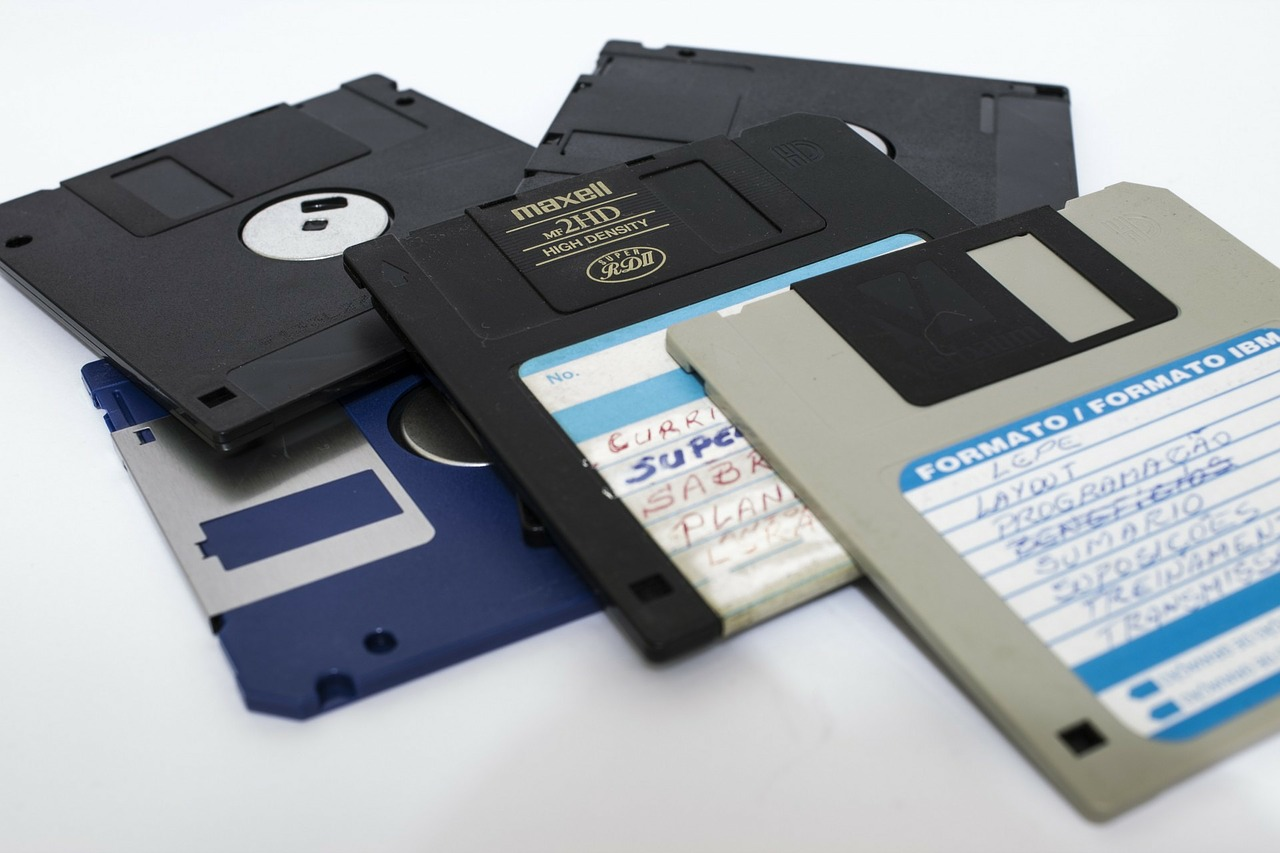
\includegraphics[width=8cm]{images/floppy-disk.jpg}
\end{figure}

Inventée dans les années 1970, elle remplaçait les cartes perforées. Quelques exemples de supports amovibles :
\begin{enumerate}
\item[] 1970 : disquette 8’’ : 1,2 Mo
\item[] 1970 : disquette 5,25’’ 360k
\item[] 1980 : disquette 3,5’’: 1,44 Mo, le standard pendant 20 ans !
\item[] 1990 : CD-ROM 700Mo (d’autre déclinaison jusqu’à 800Mo)
\item[] 1990 : ZIP : 700Mo
\item[] 2004 : DVD-ROM : 4,7 Go
\item[] 2004 : DVD-ROM double couche : 9,4 Go
\item[] 2006 : Blu-ray 25Go
\item[] 2006 : Blu-ray double couche 50Go
\item[] 2000 : clé USB et carte mémoire
\end{enumerate}

\subsection{Supports distants}
Depuis 2010, plusieurs entreprises offrent un service de stockage et de partage de fichiers dans le cloud (ou nuage). Il est donc nécessaire d’avoir une connexion Internet pour accéder à ces espaces de stockage.

\begin{remarques}
Le terme « cloud » est une forme abrégée de « cloud computing » ou l’informatique en nuage. Un cloud est constitué de serveurs situés à distance et accessibles de n’importe où et à n’importe quel moment via une connexion Internet sécurisée et protégée.
\end{remarques}

\begin{figure}[ht!]
\centering
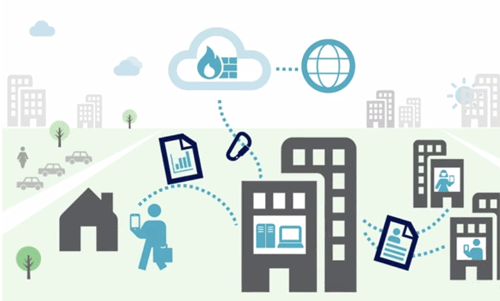
\includegraphics[width=8cm]{images/Business_Network_Solutions_swisscom.png}
\end{figure}

Quels sont les avantages et les inconvénients d’avoir ses données dans un cloud qui ne vous appartient pas (dont vous ne gérez pas l’infrastructure) ?

\begin{example} Vous prenez un contrat chez l’entreprise Tartempion 5 chf par mois pour 1 To de place pour vos données.
\end{example}

\textbf{Avantages principaux du cloud :}
\begin{enumerate}
\item[+] Vos données sont accessibles partout, à condition d’être connecté à Internet. Vos données sont donc accessibles depuis votre smartphone, votre PC, etc.
\item[+] Possibilité de partager ses données. De plus, certains logiciels permettent la modification simultanée et gèrent l’accès concurrent.
\item[+] Aucun investissement ni installation préalable requise, juste le prix de l’abonnement. Il vous suffit en général d’un navigateur web pour accéder à vos données.
\item[+] Maintenance, sécurisation des données et mises à jour effectuées par le fournisseur.
\item[+] Souplesse dans l’espace loué. Si vous avez besoin de 2 To, vous pourrez évoluer votre abonnement.
\item[+] En cas de panne de votre ordinateur personnel, vous ne perdez pas les données qui sont dans le cloud.
\end{enumerate}
\textbf{Inconvénients principaux du cloud :}
\begin{enumerate}
\item[-] Pas de contrôle total d’accès aux données par rapport à l’entreprise Tartempion. Confidentialité des données compromise si aucun outil n’est mis en place pour protéger les documents sensibles ;
\item[-] Savez-vous où sont réellement hébergées vos données ?
\item[-] Dépendance avec l’entreprise. Si Tartempion fait faillite que se passe-t-il ?
\item[-] Risque de cyberattaques si les données ne sont pas bien protégées.
\item[-] Obligation d’être connecté à Internet. Le service peut être dégradé si la liaison n’est pas fiable.
\item[-] Accès aux fichiers plus lents que sur un support local.
\item[-] Impact écologique : par ses serveurs nécessaires au fonctionnement du cloud, ce dernier induit une consommation d’énergie croissante.

\end{enumerate}

\section{Stratégie de sauvegarde}
\subsection{Introduction}
Aucun support de stockage n’a une durée de vie illimitée et aucun support de stockage n’est fiable à 100\%. Le risque zéro n’existe pas. Une perte de données numériques est donc très vite arrivée. Les causes principales sont:
\begin{enumerate}
\item[o] des défaillances techniques matérielles comme un disque dur en panne ou une clé usb qui n’est plus accessible;
\item[o] des défaillances logicielles comme un fichier corrompu suite à une écriture erronée par le système d’exploitation, une erreur de synchronisation;
\item[o] des défaillances humaines comme un fichier effacé, un fichier écrasé ou une clé usb perdue;
\item[o] des catastrophes naturelles comme des incendies ou des dégâts des eaux;
\item[o] des programmes malveillants et des attaques de virus ou de ransomware;
\item[o] le vol du matériel comme votre téléphone portable, un disque d’un serveur, une clé usb, une carte mémoire;
\end{enumerate}
Le monde professionnel indique une durée de vie moyenne de 5 ans pour un disque dur mécanique ou un disque type SSD. Une clé usb ou une carte mémoire de qualité pourrait tenir 10 ans. Le cloud offert par les entreprises de stockage a une durée de vie quasi illimitée, du moins celle de l’entreprise.

\subsection{Stratégie 3-2-1 de sauvegarde de données}

La stratégie de sauvegarde 3-2-1 représente le b-a-ba et le minimum de la protection des données. Mise au point par un photographe souhaitant protéger ses clichés dans les années 1920, cette stratégie est devenue une référence, car elle permet une protection optimale des données, quel que soit leur format.

Le concept de base de la stratégie 3-2-1 repose sur trois principes :
\begin{enumerate}
    \item[->] \textbf{{\huge 3} copies de vos données:} La stratégie recommande d’avoir 2 copies plus la source. Avec trois copies dont deux sauvegardes, le risque que les trois copies aient un problème en même temps est très faible surtout si elles sont stockées sur des supports différents.

    \item[->] \textbf{{\huge 2} supports différents:} La notion de supports différents est essentielle quand on parle de données numériques, car quel est l’intérêt d’avoir deux sauvegardes si elles sont stockées sur le même support ? En cas d’incident, toutes les données seraient perdues. Il est donc important que la source et au moins une de ses copies soient sauvegardées sur des supports différents.

    \item[->] \textbf{{\huge 1} copie hors site:} Quel que soit le support (NAS, disque dur externe, lecteur de bande, etc.), aucune stratégie de sauvegarde de données numériques ne peut être considérée comme sûre si au moins une des copies n’est pas stockée « hors site ». Le récent incendie du 10 mars 2021 d’OVH en est la preuve. En effet, certains utilisateurs avaient leur site en production sur un serveur et leurs copies sur un autre serveur. Certes, les copies étaient sur des supports différents, mais elles étaient stockées dans le même datacenter. Comme une grande partie du site contenant ces serveurs a cessé de fonctionner à cause de l’incendie, aucune des copies n’était utilisable. Or, si au moins une de ces copies avait été stockée chez un autre hébergeur (hors site), ces utilisateurs auraient pu rétablir rapidement leurs services.
\end{enumerate}

Malgré tout les stratégies de sauvegarde ont leurs limites ! La quantité de données à sauvegarder peut prendre trop de temps et poser des problèmes d’intégrité des données. L’externalisation des sauvegardes selon la méthode 3-2-1 soulève aussi la question de la protection des données. 

Et si vous avez bien conservé votre donnée numérique. Serez-vous capable de la relire ?

\section{Compression des données}


\section{Exercices}

\begin{exercice}
En réfléchissant aux derniers cours, essayez de calculez la taille que ferait un fichier texte \texttt{blabla.txt} contentant la chaîne de caractères \texttt{blablabla}.
Vérifiez ensuite en le créant sur votre ordinateur.
\end{exercice}


\begin{exercice}
Reprenez le dossier \texttt{Nourriture} de l'exercice 2 du chapitre précédent. Compressez-le et comparez sa taille originale avec sa taille une fois compressé.
\end{exercice}

\begin{exercice}
Téléchargez l'image \texttt{sample\_1920x1280.bmp} en haute définition depuis moodle puis convertissez-la dans les formats suivants en comparant la taille et la qualité de l'image à chaque étape. 

\textit{Utilisez par exemple le site \url{https://online-converting.com/image} pour faire la conversion en jpg et \url{https://online-converting.com/image/convert2bmp} pour le bmp}
\begin{center}
   \begin{tabular}{| l || c | r | }
     \hline
     Format & Taille (ko) & Qualité visuelle \\ \hline
     .bmp en 24 bits &  &  \\ \hline
     .bmp en 8 bits &  &  \\ \hline
     .jpg &  &  \\ \hline
     .png &  &  \\
     \hline
   \end{tabular}
\end{center}
\end{exercice}


\end{document}